\documentclass{beamer}
\usepackage{amsmath,amssymb,amsthm,array}
\usepackage{bm}
\usepackage{xltxtra}
\usepackage{multirow}
\usepackage{multicol}
\usepackage{algorithm}
\usepackage{algorithmic}
\usepackage[normalem]{ulem}
\usetheme{CambridgeUS}
\usecolortheme{dolphin}
\setmainfont[Mapping=TeX-text]{GFS Neohellenic}
\usefonttheme{serif}
\setbeamertemplate{navigation symbols}{}
\title{Homomorphic Voting Based on Paillier Cryptosystem}
\author{Panagiotis Grontas}
\date{26/06/2013}
\defbeamertemplate*{footline}{shadow theme}
{%
  \leavevmode%
  \hbox{\begin{beamercolorbox}[wd=.5\paperwidth,ht=2.5ex,dp=1.125ex,leftskip=.3cm plus1fil,rightskip=.3cm]{author in head/foot}%
    \usebeamerfont{author in head/foot}\insertframenumber\,/\,\inserttotalframenumber\hfill\insertshortauthor (\insertshortinstitute)
  \end{beamercolorbox}%
  \begin{beamercolorbox}[wd=.5\paperwidth,ht=2.5ex,dp=1.125ex,leftskip=.3cm,rightskip=.3cm plus1fil]{title in head/foot}%
    \usebeamerfont{title in head/foot}\insertshorttitle%
  \end{beamercolorbox}}%
  \vskip0pt%
}
\institute{$\mu\Pi\lambda\forall$  - CoReLab Crypto Group}


\setlength{\columnseprule}{0.4pt}
\begin{document}
\newcommand{\zns}[1]{ \mathbb{Z}_{#1}^* }
\newcommand{\md}[1]{\quad (mod \, {#1})}
\begin{frame}
\titlepage
\end{frame}

\section{Introduction}

\begin{frame}{Motivation}
\begin{itemize}
\item Homomorphic property $E(v1) \otimes E(v2) = E(v1 \oplus v2)$
\item In voting: Count the votes while maintaining secrecy
\item Exponential ElGamal: $E(v,r) = (g^r, g^m  h^r)$ instead of $(g^r, m  h^r)$
\item Decryption has to solve discrete log problem
\begin{itemize}
	\item Not as bad as it sounds
	\item Difficulty depends on the message space
	\item Problem on elections with multiple candidates
\end{itemize}
\item Solutions based on quadratic or higher residuosity
\end{itemize}
\end{frame}

\section{Paillier Cryptosystem}

\begin{frame}{Key Generation} 
\begin{itemize}
\item Choose two large primes $p,q$ randomly and independently such that $gcd(p  q,(p-1)  (q-1))=1$
\item Calculate RSA modulus $ n = pq $ 
\item Calculate $ \bm{\lambda} = lcm(p-1,q-1)= \frac{(p-1)  (q-1)}{gcd(p-1,q-1)} $ (Carmichael's Function)
\begin{itemize}
	\item Easy to calculate if we know $p,q$
	\item $ \forall x \in \mathbb{Z}_{n^2}: x^{\lambda(n)} =  1 \quad mod n $
	\item $ \forall x \in \mathbb{Z}_{n^2}: x^{n  \lambda(n)} =  1 \quad mod n^2 $
\end{itemize}
\item Select generator $g \in \mathbb{Z}^{*}_{n^2}$
\begin{itemize}
	\item The order of $g$ must be a non zero multiple of $n$
\end{itemize}
\item Calculate inverse  $\bm{\mu} = L(g^\lambda \, ( mod \, n^2 ) )^{-1} \, mod \, n$  where  $L(x) = \frac{x-1}{n} $
\begin{itemize}
\item $L()$ is given elements that are equal to $1 \quad mod n$
\item $L()$ \textit{'solves'} the discrete log problem and \textit{'decrypts'}
\item Inverse always exists if g is a valid generator
\end{itemize}
\item Public Key is $(n,g)$ and private Key $(\lambda,\mu)$ 
\begin{itemize}
	\item We can always select $g = n+1$ so public key becomes $n$
\end{itemize}
\end{itemize} 
\end{frame}

\begin{frame}{Operation}
\begin{block}{Encryption}
\begin{itemize}
\item Encode message $m$ into $\mathbb{Z}_n$
\item Select random $r \in \mathbb{Z}^*_n$
\item Return $c = E_{g}(m,r) = g^m  r^n \, ( mod \, n^2 )$
\end{itemize}
\end{block}

\begin{block}{Decryption}
\begin{itemize}
\item Ciphertext $c \in \mathbb{Z}^*_{n^2}$
\item Return $m = L(c^\lambda \, mod \, n^2)  \mu \, ( mod \, n) = \frac{L(c^\lambda \, mod \, n^2)}{L(g^\lambda \, mod \, n^2)} (mod n) $
\end{itemize}
\end{block}

\end{frame}

\begin{frame}{Security}

\begin{block}{The composite residuosity problem}
\begin{itemize}
\item Given $n=p  q$ and $z \in \mathbb{Z}^*_{n^2}$ decide if $z$ is $n-residue$ module $n^2$
\item Does there exist $y \in \mathbb{Z}^*_{n^2}$ st: $z = y^n (mod n^2)$
\end{itemize}
\end{block}

\textbf{Decisional composite residuosity assumption (DCRA)}: There is no polynomial time algorithm to decide the composite residuosity problem. \\

\textbf{Remark}: If there was an algorithm to decide if $z \in \mathbb{Z}^*_{n^2}$ is the encryption of message $0$ then we could solve the composite residuosity problem

\end{frame}

\begin{frame}[allowframebreaks]{Correctness}

\begin{block}{Target}
Prove that for $c = E_{g}(m,r) = g^m  r^n (mod n^2)$ \\
the decryption operation $ \frac{L(c^\lambda \, mod \, n^2)}{L(g^\lambda \, mod \, n^2)} (mod n)$ yields $m$.
\end{block}

\begin{block}{Main Lemma}
$\forall \, w \, \in Z^*_{n^2}:  \bm{L(w^\lambda \,mod \, n^2) = \lambda [w]_{n+1} \, mod \, n}$ 
\end{block}

\begin{block}{Notation}
\begin{itemize}
\item $w=E_{n+1}([w]_{n+1},r)$ which means $w$ is the ciphertext and $[w]_{n+1}$ is the plaintext for $g=n+1$
\item $\lambda = lcm(p-1,q-1)$
\item $ L(x) = \frac{x-1}{n} $  
\end{itemize}
\end{block}

\begin{block}{Helper Lemma 1}
$ \forall x \in \mathbb{Z}_n : (1+n)^x = 1 + n  x  \,\, (\, mod \, n^2) $ 
\end{block}

\begin{Proof}
\begin{flalign*}
(1+n)^x = \\
1 + {x \choose  1}  n + {x \choose  2}  n^2 + s  + n^x  \,\, (\, mod \, n^2) =\\
1 + x  n	\,\, (\, mod \, n^2)
\end{flalign*}
\end{Proof}

\begin{block}{Helper Lemma 2}
$ \forall c \in \mathbb{Z}_{n^2}^*, $ and proper generators $g_1,g_2$   : $\quad [c]_{g_1} = [c]_{g_2}  [g_2]_{g_1} $
\end{block}

\begin{Proof}
\begin{flalign*}
g_2  = g_1^y  b^n      \quad \quad 	\sim       \quad \quad y = [g_2]_{g_1} \\
c = g_2^z  d^n 		\quad \quad 	\sim       \quad \quad z = [c]_{g_2} \\
c = g_2^z  d^n  = (g_1^y  b^n)^{z}  d^n = g_1^{zy}   (b^z  d) ^n  \quad \quad \sim       \quad \quad y  z = [c]_{g_1} \\
[c]_{g_1} = [c]_{g_2}  [g_2]_{g_1}
\end{flalign*}
\end{Proof}

\begin{block}{Main Lemma Proof}
$\forall \, w \, \in Z^*_{n^2}:  \bm{L(w^\lambda \,mod \, n^2) = \lambda [w]_{n+1} \, mod \, n}$ \\
$n+1$ is a proper generator g \\
$\forall \, w \, \in Z^*_{n^2}:$ \\
\begin{flalign*}
w=E_{n+1}([w]_{n+1},r)=(n+1)^{[w]_{n+1}}  r ^ n \, (mod n^2) \Rightarrow \\
w^\lambda 	= (n+1)^{\lambda  [w]_{n+1}}  r ^ {\lambda  n} \, (mod n^2)  \\
     		= \bm{(1 + \lambda  [w]_{n+1}  n)}  r ^ { \bm {k  \phi(n)}  n} \, (mod n^2)  \\
     		= (1 + \lambda  [w]_{n+1}  n)  \\
L(w^\lambda) = \frac {w^\lambda - 1} { n }= \lambda  [w]_{n+1}
\end{flalign*}

\end{block}


\begin{block}{Decryption operation:}
\begin{flalign*}
\frac{L(c^\lambda \, mod \, n^2)}{L(g^\lambda \, mod \, n^2)} = \\
\frac{ \lambda  [c]_{n+1} }{ \lambda  [g]_{n+1}} = \\
\frac{    [c]_{n+1} }{   [g]_{n+1}} = 
\frac{    [c]_{g}  [g]_{n+1} }{   [g]_{n+1}} = [c]_{g} = m
\end{flalign*}
\end{block}

\end{frame}

\begin{frame}{Homomorphic Properties}
\begin{itemize}
\item $D(E_{g}(m_1,r_1)  E_{g}(m_2,r_2)) = m_1+m_2 \quad mod \, n$
\item $D(E_{g}(m_1,r_1)  g^{m_2}) = m_1+m_2 \quad mod \, n$ (a full encryption of the second message is not necessary)
\item $D(E_{g}(m_1,r_1)  g^{nx}) = m_1+nx \quad mod \, n = m_1 $ (self blinding)
\item $D(E_{g}(m_1,r_1)^k) = k  m_1$ 
\end{itemize}
\end{frame}

\begin{frame}[allowframebreaks]{A Generalisation \cite{Damgard:2001:GSA:648118.746742}}

For each $s \geq 1$ we can define a cryptosystem $CS_s$:

\begin{block}{Key Generation}
\textbf{Input:} security parameter $k$
\begin{itemize}
\item Select admissible $n = p  q$ with length $k$ bits
\item Choose random $j$ with $gcd(j,n)=1$ and random $x \in \mathbb{Z}_{n^s}$ and calculate $ g = (1+n)^j  x \quad mod n^{s+1}$
\item Calculate $\lambda = lcm(p-1,q-1)$
\item Select $d$ such that
\begin{itemize}
\item $d \, mod \, n \in \mathbb{Z}^{*}_{n^s}$
\item $d = 0 \quad (mod \lambda)$
\end{itemize}
\end{itemize}
\textbf{Output:} Public key = $(n,g)$ Private key = $d$ \\
\emph{Remark:} Paillier Cryptosystem is the special case $s = 1$ \\
In Paillier $d = \lambda$ but larger values are preferred for threshold version to be secure.
\end{block}

\begin{block}{Encryption}
\begin{itemize}
\item Encode message $m$ into $\mathbb{Z}_{n^s}$
\item Select random $r \in \mathbb{Z}^*_n$
\item Return $c = E_{g}(m,r) = g^m  r^{n^s} \, ( mod \, n^{s+1} )$
\end{itemize}
\end{block}

\begin{block}{Decryption}
\begin{itemize}
\item Ciphertext $c \in \mathbb{Z}^*_{n^{s+1}}$
\item Calculate $c^d \quad mod n^s = (1+n)^{m  j  d} \quad mod n^s  $
\item Extract $m  j  d$
\item Calculate $g^d \quad mod n^s = (1+n)^{ j  d} \quad mod n^s  $
\item Extract $ j  d$
\item $ m =\frac{m  j  d}{j  d}$
\end{itemize}
\end{block}

\begin{block}{Security}
$\forall s$ $CS_s$ is one way if Paillier ($CS_1$) is one way and semantically secure iff the DCRA is true
\end{block}

\end{frame}

\begin{frame}[allowframebreaks]{A simplification}

\begin{block}{Key Generation}
\begin{itemize}
\item Public key is $n=p  q$
\item Private key is $\lambda = lcm (p-1, q-1)$
\end{itemize}
$g = (1+n)$ and $s$ can be selected at any point in time as long as $ m < n^s$
\end{block}

\begin{block}{Encryption}
\begin{itemize}
\item Encode message $m$ into $\mathbb{Z}_n$
\item Select random $r \in \mathbb{Z}^*_n$
\item Return $c = E(m,r) = (1+n)^m  r^{n^s} \, ( mod \, n^{s+1} )$
\end{itemize}
\end{block}

\begin{block}{Decryption}
\begin{itemize}
\item Ciphertext $c \in \mathbb{Z}^*_{n^2}$
\item Calculate $c^\lambda mod n^{s+1} = (1+n)^{m  \lambda \, mod n^s}  r^{\lambda  n^s) \, mod \lambda} \quad mod n^{s+1} = (1+n)^{m  \lambda} \quad mod n^{s+1} $
\item  Extract $m  \lambda$
\item  $ m = \frac{m  \lambda}{\lambda}$
\end{itemize}
\end{block}

\begin{block}{Security}
$\forall s$ the simplified version is one way if Paillier ($CS_1$) is one way and semantically secure iff the DCRA is true.
\end{block}

\end{frame} 

\section{Threshold Paillier}

\begin{frame}[allowframebreaks]{Threshold decryption: a reminder}
\begin{center}
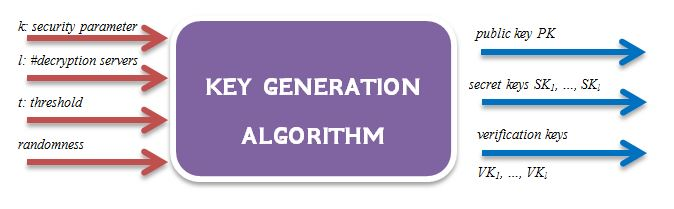
\includegraphics[scale=0.35]{threshold1.jpg}
\end{center}
\begin{center}
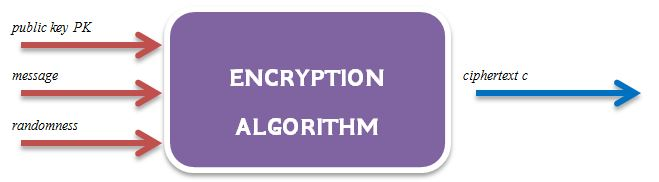
\includegraphics[scale=0.35]{threshold2.jpg}
\end{center}
\begin{center}
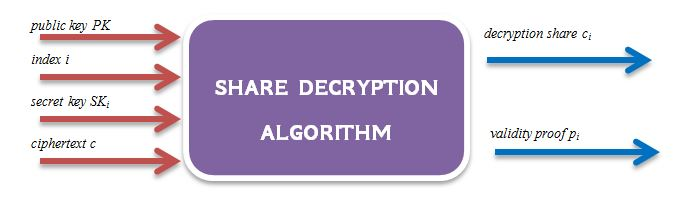
\includegraphics[scale=0.35]{threshold3.jpg}
\end{center}
\begin{center}
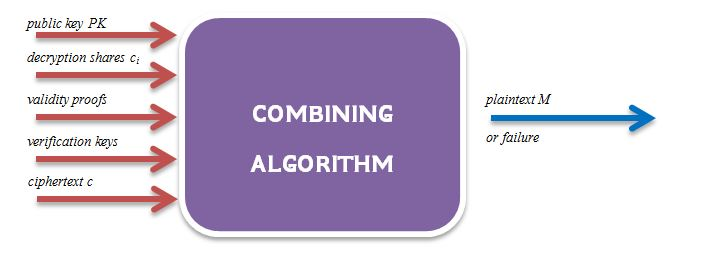
\includegraphics[scale=0.35]{threshold4.jpg}
\end{center}
\end{frame}

\begin{frame}{Reminder:Shamir secret sharing}
\begin{block}{Objective}
Share a secret element $s$ between $l$ players so that any $t+1$ subset can recover it, but no $t$ element subset can.
\end{block}
\begin{itemize}
\item Main:Idea Lagrange Interpolation
\item A polynomial $P$ of degree $t$ can be reconstructed from $t+1$ distinct elements $(x_i, y_i)_{i=1}^{t+1}$
\item $P(x) = \sum_{i=1}^{t+1} \prod_{j=1,j \neq i}^{t+1} \frac{x-x_j}{x_i - x_j}  y_i$  
\item To share a secret:
\begin{itemize}
\item Dealer chooses a random polynomial of degree $t$ so that $P(0) = s$
\item Distribute $l$ pairs $(x_i,P(x_i)) x_i \neq 0$
\item $t+1$ players can reconstruct the polynomial (and recover $s$), but $t$ players cannot
\end{itemize}
\end{itemize}
\end{frame}

\begin{frame}{Reminder:Proof of Discrete Log Equality}
\begin{block}{$Proof(a,b,A,B)$}
$a$, $b$ are elements of a cyclic group $G$ with generator $g$, \\ 
Prove that $A,B$ have the same logarithm $s$ in bases $a,b$
\end{block}
How \textit{(Non Interactive Version)}
\begin{itemize}
\item Select a random element $r \in G$
\item Calculate $x_a = a^r$ and $x_b = b^r$
\item Generate $e = hash(a,b,A,B,x_a,x_b)$ 
\item Calculate $t = r+e  s$
\item Calculate $e' = hash (a,b,A,B, \frac{a^t}{A^e}, \frac{b^t}{B^e} )$
\item Check if $e=e'$
\end{itemize}
\end{frame}

\begin{frame}[allowframebreaks]{Threshold RSA \cite{Shoup:2000:PTS:1756169.1756190}}
\begin{itemize}
\item \textbf{Key Generation}
\begin{itemize}
\item Calculate RSA modulus $n = p  q$ where $p=2p'+1, q=2q'+1$ and $m=p'  q'$. Notice that $4  m = \phi(n)$
\item Choose prime $e>l$
\item Choose $d \in \mathbb{Z}_m$ st: $ e  d = 1 \quad mod m$
\item Share $d$ using Shamir Secret Sharing
\begin{itemize}
\item Polynomial $ f(x) = \sum_{i=0}^t f_i  x^i $
\item $f_0 = d$
\item $f_i \in_R \mathbb{Z}_m$
\end{itemize}
\item Secret Shares: $SK_i = d_i = f(i) \quad mod m$  
\item Verification Keys:
\begin{itemize}
\item $Q_n =  \{ x \in \zns{n} | x=y^2 \md{n}  \} $
\item $VK = v \in_R Q_n$ and 
\item $VK_i = v^{d_i} \md{n} $ 
\end{itemize}
\end{itemize}

\framebreak
\item \textbf{Encryption}
\begin{itemize}
\item $E(M) = M^e  \md{n}$
\end{itemize}
\item \textbf{Decryption shares}
\begin{itemize}
\item Calculate $\Delta = l!$
\item Decryption shares: $c_i = c^{2  \Delta  d_i} $
\item Validity Proof $Proof( c^{4  \Delta}, v, c_i^2 = (c^{4  \Delta})^{d_i}   , v^{d_i})$
\end{itemize}
\item \textbf{Combination Preliminaries}
\begin{itemize}
\item Validate proofs of decryption shares.
\item If $t$ shares are valid at most then fail.
\item Set $S$ a set of $t+1$ valid decryption shares
\item Lagrange coefficients multiplied by $\Delta$: 
$\mu^S_{i,j} = \Delta  \frac{\prod_{j'} (i-j')}{\prod_{j'} (j-j')}$
$\mu^S_{0,j} = \Delta  \frac{\prod_{j'} ( -j')}{\prod_{j'} (j-j')}$
\item $\Delta  f(i) = \sum_{j} \mu^S_{i,j}  f(j) \md{m}$
\end{itemize}

\framebreak

\item \textbf{Combination Algorithm}:Retrieve $d=f(0)$ and decrypt 

\begin{itemize}
\item Raise squares of shares $c_j$ to $\mu^S_{0,j}$ for $j \in S$ 
\item Create product of above 
  
\begin{center}
$ 
 w = \prod_j c_j^{2  \mu^S_{0,j}}    
   = \prod_j c^{(2  \Delta  d_j)  (2  \mu^S_{0,j}) }  
   = \prod_j (c^{4  \Delta})^{d_j  \mu^S_{0,j}}  
   = (c^{4  \Delta})^{\sum_j d_j  \mu^S_{0,j}}  
   = (c^d)^{4  \Delta^2} 
   = M^{4  \Delta^2} 
$  
  
\end{center}
\item Using EGCD calculate $a,b$ st: $a  4\Delta^2 + b  e =1$
\item Calculate $w^a= M^{4  \Delta^2  a}$
\item Calculate $c^b = M^{e  b}$
\item $M^{4  \Delta^2}  M^{e  b} = M$
\end{itemize}
\end{itemize}
\end{frame}

\begin{frame}[allowframebreaks]{Threshold Paillier \cite{fouque2001sharing}}
\begin{itemize}
\item \textbf{Key Generation}
\begin{itemize}
\item Calculate RSA modulus $n = p  q$ with $gcd(n,\phi(n))=1$ where $p=2p'+1, q=2q'+1$ and $m=p'  q' = \frac{p-1}{2}  \frac{q-1}{2}$ 
\item Generate g
\begin{itemize}
\item Randomly choose $(a,b) \in \zns{n} \times \zns{n}$ 
\item Set $g=(1+n)^\alpha  b^n \md{n^2}$
\end{itemize}
\item Choose random element $\beta \in \zns{n}$
\item Set secret key $SK=\beta  m$ 
\item Shamir secret key sharing
\begin{itemize}
\item $f_0 = SK$
\item Coefficients $f_i \in_R \{0, s, n  m - 1 \}$ 
\item Polynomial $f(x) = \sum_{i=0}^t f_i  x^i \md{nm}$
\item Shares $ s_i = f(i) \md{nm} $
\end{itemize}
\item Public Key
\begin{itemize}
\item $\theta = L(g^{m  \beta}) = a  m  \beta \md{n}$
\item $(n,g,\theta)$
\end{itemize}
\item Verification Keys:
\begin{itemize}
\item $Q_n =  \{ x \in \zns{n} | x=y^2 \md{n}  \} $
\item $VK = v \in_R Q_n$ and 
\item $VK_i = v^{d_i} \md{n} $ 
\end{itemize}
\end{itemize}
\item \textbf{Encryption}
\begin{itemize}
\item $r \in_r \zns{n}$
\item $E(M) = g^M  r^N  \md{n^2}$
\end{itemize}
\item \textbf{Share Decryption}
\begin{itemize}
\item $\Delta = l!$
\item Decryption shares: $c_i = c^{2  \Delta  s_i} \md{n^2}$
\item Validity Proof $Proof( c^{4  \Delta}, v^\Delta, c_i^2 = (c^{4  \Delta})^{s_i}   , v^{s_i})$
\end{itemize}
\framebreak
\item \textbf{Combination Preliminaries}
\begin{itemize}
\item Validate proofs of decryption shares.
\item If $t$ shares are valid at most then fail.
\item Set $S$ a set of $t+1$ valid decryption shares
\item Lagrange coefficients multiplied by $\Delta$: 
\item $\mu^S_{i,j} = \Delta \frac{\prod_{j'} (i-j')}{\prod_{j'} (j-j')}$
\item $\mu^S_{0,j} = \Delta  \frac{\prod_{j'} j'}{\prod_{j'} (j-j')}$
\item $\Delta  f(0) = \sum_{j} \mu^S_{0,j}  f(j) mod m$
\end{itemize}
\framebreak
\item \textbf{Combination Algorithm}
\begin{itemize}
\item Raise squares of shares $c_j$ to $\mu^S_{0,j}$ for $j \in S$ 
\item Create product of above 
\item 
\begin{center}
$ 
 w = \prod_j c_j^{2  \mu^S_{0,j}}    
   = \prod_j c^{(2  \Delta  s_j)  (2  \mu^S_{0,j}) }  
   = \prod_j (c^{4  \Delta})^{s_j  \mu^S_{0,j}}  
   = (c^{4  \Delta})^{\sum_j s_j  \mu^S_{0,j}}  
   = (c^{m  \beta})^{4  \Delta^2} 
$
\end{center}
\item But $c$ is a Paillier encryption of message M. $c = g^M  r^N$
\begin{center} 
$
(c^{m  \beta})^{4  \Delta^2} = ((g^M  r^n)^{m  \beta})^{4  \Delta^2} =  
(1+n)^{a  4  \Delta^2  m  \beta  M}  (b  r) ^ {n  m  \beta  4  \Delta^2} \md{n^2} =   
(1+n)^{a  4  \Delta^2  m  \beta  M} \md{n^2} =  
 1+n  a  4  \Delta^2  m  \beta  M  \md{n^2}
$
\end{center}
\item Apply L function: $L(1+n  a  4  \Delta^2  m  \beta  M) = a  4  \Delta^2  m  \beta  M = M  4  \Delta^2  \theta$

\item Divide by $4  \Delta^2  \theta$ (public information) and retrieve plaintext $M$.
\end{itemize}
\end{itemize}

\begin{theorem}
If the original Paillier cryptosystem is semantically secure then the threshold version is secure as well.
\end{theorem}

\end{frame}

\section{Zero Knowledge Proofs}

\begin{frame}[allowframebreaks]{Proof of Knowledge Of Randomness}
\begin{block}{Objective}
The prover presents a ciphertext $c$ to the verifier and claims that it encrypts the message $m$, which means that the prover possesses randomness $r$ st: 
$c = E(m,r)$
\end{block}
\begin{align*}
c = E(m,r) = g^m r^{n^s} \md{n^{s+1}} \Rightarrow \\
c g^{-m} = r^{n^s} \md{n^{s+1}} \Rightarrow \\
c g^{-m} = E(0,r)
\end{align*}
We must prove that $c g^{-m}$ is a $n^s$ power \\
\uline{\textbf{The protocol}}
\begin{center}
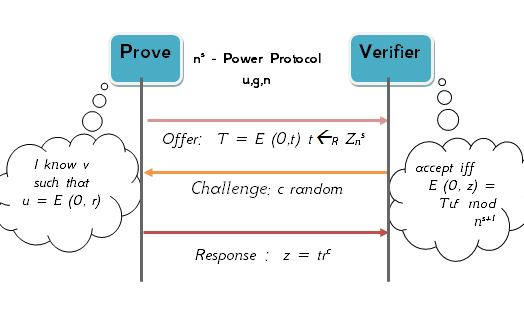
\includegraphics[scale=0.50]{ns-power.jpg}
\end{center}

\uline {Completeness:} $E(0,z) = E(0,rv^e) = E(0,r) E(0,v^e) = E(0,r) E(0,v)^e = a u^e \md{n^{s+1}}$
\end{frame}


\section{Voting with Paillier}
 
\begin{frame}[allowframebreaks]{Homomorphic Tallying \cite{Damgard03ageneralization}}
\begin{block}{Yes-No Voting}
\begin{itemize}
\item There are $M$ voters
\item Each voter decides on his vote $v_i$ and calculate $E_i = E(v_i,r_i)$
\item Compute ZK Proof of validity
\item The authority(-ies) filter out the votes with invalid proofs
\item Compute $E=\prod_{i}E_i=E(\sum_{i}v_i \quad mod n^2, \prod_{i}r_i \mod n)$
\item The authority decrypts and receives the number of yes-votes $\sum_{i}v_i $
\item The number of no-votes can be computed by subtracting from the total-number of valid votes.
\item Remark: The tally must be less than $n^2$
\item There are generalisations of Paillier for $n^s, s \geq 2$. One can choose $s$ such that $M<n^s$
\end{itemize}
\end{block}

\begin{block}{$L>2$ candidates - A simple solution}
\begin{itemize}
\item $L$ parallel yes/no votes $v_{ij}$
\item $v_{ij} = 1$ for the preferred candidates
\item Proof of validity must include that the voter voted for exactly $t$ candidates
\item $L$ parallel sums
\item \textbf{Remarks}: 
\begin{itemize}
\item The vote size is large $O(L  log_{2}n)$
\item Many decryptions are needed
\end{itemize}
\end{itemize}
\end{block}

\begin{block}{$L>2$ candidates - A better solution \cite{Damgard03ageneralization}}
\begin{itemize}
\item Vote for candidate $j$ - Encryption of $M^j$
\item Vote for $t$ candidates: Submit many encryptions
\item $M^L < n^s$
\item Tallying: All encrypted votes are multiplied
\item The result is of the form $a = \sum a_j M^j$ where $a_j$ is the number of votes cast for candidate $j$ 
\item The result is a number in $M-ary$ notation
\begin{itemize}
\item The vote size is   $O(log_2L  log_{2}n)$
\item One decryption is needed
\item An extra proof must be employed to deter voting for the same candidate $t$ times
\end{itemize}
\end{itemize}
\end{block}


\end{frame}

\begin{frame}[allowframebreaks]{References}
\begin{small}
\nocite{*}
\bibliographystyle{alpha}
\bibliography{paillier}
\end{small}
\end{frame}

 
\end{document}
